\chapter{Introdução}
\label{Introducao}

Neste trabalho vamos estudar algoritmos sobre matrizes Monge e matrizes com propriedades parecidas, como a monotonicidade total e a monotonicidade. As matrizes Monge foram estudadas inicialmente em 1781 por Gaspard Monge~\cite{Monge:1781}. Ghys~\cite{Ghys:2012} escreveu um bom artigo sobre os estudos realizados por Monge. O problema pelo qual Monge se interessou consiste de duas regiões de igual área no plano. Em uma das regiões, há terra. O objetivo é transportar toda a terra desta para a outra região podendo dividir tal área em infinitas partes de forma a minimizar a soma, para cada porção de terra, do produto de sua área por sua distância percorrida. É interessante notar que Monge estudou também a versão em 3 dimensões deste problema.

Ao estudar este problema, Monge realizou uma primeira observação simples, porém muito importante. Se duas partículas de terra, uma inicialmente em um ponto~$A$ e a outra em um outro ponto~$B$, forem enviadas, respectivamente, para os pontos~$b$ e~$a$, então os caminhos entre~$A$ e~$b$ e~$B$ e~$a$ não podem se cruzar em uma solução ótima. Se estes caminhos se cruzassem, seria menos custoso enviar a primeira porção para o ponto~$a$ e a segunda para o ponto~$b$. Séculos mais tarde, em 1961, Hoffman~\cite{Hoffman:2003} utilizou esta propriedade ao estudar problemas de transporte e creditou sua descoberta a Monge, cunhando o termo ``Propriedade de Monge''.

\begin{figure}[h]
    \centering
    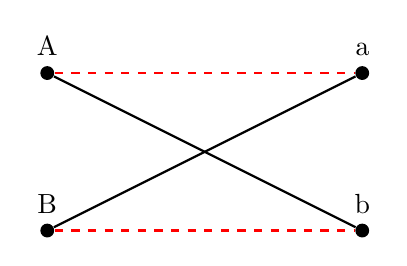
\begin{tikzpicture}
  \tikzset{dot/.style 2 args={circle,fill=#1,inner sep=0,minimum size=5pt,label={above:#2}}}
  \node[dot={black}{A}] (A) at (0,2) {};
  \node[dot={black}{B}] (B) at (0,0) {};
  \node[dot={black}{a}] (a) at (4,2) {};
  \node[dot={black}{b}] (b) at (4,0) {};

  \draw[thick,black] (A) -- (b);
  \draw[thick,black] (B) -- (a);
  \draw[thick,dashed,red] (A) -- (a);
  \draw[thick,dashed,red] (B) -- (b);
\end{tikzpicture}

    \caption{Desigualdade quadrangular. A soma dos tamanhos dos segmentos em preto é maior do que a soma dos tamanhos dos segmentos pontilhados em vermelho.} \label{Introducao:QI}
\end{figure}

Como a Figura~\ref{Introducao:QI} indica, a propriedade de Monge possui uma interpretação geométrica simples e interessante: em um quadrilátero convexo, a soma dos tamanhos das diagonais supera a soma dos tamanhos de dois lados paralelos. Uma forma de modelar esta propriedade é a criação de matrizes Monge. Grande parte da importância das matrizes Monge é consequência de seu relacionamento natural com geometria. 

Aggarwal, Klawe, Moran, Shor e Wilber~\cite{Aggarwal:1987}, percebendo esta utilidade, estudaram as matrizes Monge e desenvolveram o algoritmo~\textsc{SMAWK} para a busca valores ótimos em linhas e colunas de matrizes totalmente monótonas. Além disso, mostraram modelagens interessantes de problemas geométricos sobre matrizes deste tipo, resolvendo tais problemas com eficiência inédita. Estas descobertas incrementaram o interesse acadêmico sobre as matrizes Monge e desencadearam uma série de artigos que demonstram a utilidade delas. Burkard, Klinz e Rudolf~\cite{Burkard:1996} compilaram muito do conhecimento desenvolvido acerca do tópico. Esta introdução, até aqui, é baseada na introdução de tal compilação.

Com algumas destas descobertas em mente, Park~\cite{Park:1991}, em sua tese, resumiu bem a motivação para o estudo das matrizes Monge. As propriedades destas matrizes permitem que certas entradas importantes sejam encontradas sem a necessidade de analisar toda a matriz e muitos problemas computacionais podem ser reduzidos a encontrar tais entradas neste tipo de matriz. A combinação destas duas afirmações faz com que estas matrizes muitas vezes permitam algoritmos especialmente eficientes para a solução de diversos problemas.

Além de suas aplicações geométricas, as matrizes Monge são úteis em diversas aplicações relacionadas a programação dinâmica~\cite{Bein:2009,Burkard:1996,Galil:1992}. Yao~\cite{Yao:1980,Yao:1982} explicitou esta relação ainda antes do desenvolvimento do algoritmo~\textsc{SMAWK}. Esta utilidade, que vai além das descobertas de Yao, fez com que as técnicas baseadas em matrizes Monge se tornassem populares em competições de programação como a Maratona de Programação e a ICPC.

Este trabalho explica alguns dos algoritmos conhecidos que se baseiam em propriedades relacionas às matrizes Monge, implementa os algoritmos estudados e exemplifica algumas aplicações dos mesmos. O Capítulo~\ref{Monge} introduz as matrizes Monge, monótonas e totalmente monótonas, introduzindo também resultados importantes sobre elas que são utilizados durante todo o texto. 

Os Capítulos~\ref{DivConq} e~\ref{SMAWK} apresentam os algoritmos para busca de valores ótimos em linhas e colunas de matrizes Monge. O Capítulo~\ref{DivConq} apresenta o método conhecido como Otimização da divisão e conquista e o Capítulo~\ref{SMAWK} apresenta o algoritmo~\textsc{SMAWK}, que já foi citado. Durante estes capítulos, é exemplificada a relação entre as matrizes Monge e programação dinâmica e alguns problemas são dados como exemplos. Um problema geométrico também é explicado e resolvido.

O Capítulo~\ref{KY} introduz a Otimização de Knuth-Yao, um método que agiliza certas soluções de programação dinâmica. Knuth~\cite{Knuth:1971} desenvolveu tal método e Yao~\cite{Yao:1980,Yao:1982} notou sua relação com as matrizes Monge. Apresentamos o método demonstrando os resultados obtidos por Yao e aplicamos o conhecimento para resolver um problema.

O Capítulo~\ref{EDPD} é focado em programação dinâmica. Ele apresenta um exemplo de solução em programação dinâmica que pode ser agilizado de maneira não trivial sem utilizar propriedades relacionadas a matrizes Monge. O objetivo deste capítulo é apresentar a possibilidade da utilização de estruturas de dados em programação dinâmica. 

O Capítulo~\ref{Online} apresenta uma estrutura de dados relacionada às matrizes Monge que é útil para agilizar algumas soluções de programação dinâmica de maneira parecida com a do Capítulo~\ref{EDPD}. O método apresentado encontra valores ótimos em linhas ou colunas de matrizes Monge onde as entradas não são todas conhecidas à priori que respeitam um certo formato. Este formato é natural para aplicações de programação dinâmica, o que demonstra o utilidade de tal técnica.

Finalmente, o Capítulo~\ref{Exemplos} documenta os exemplos de aplicações implementados que utilizam os algoritmos estudados e o Capítulo~\ref{Subjetiva} contém uma apreciação subjetiva do autor acerca do trabalho.

\section{Conteúdo}
O conteúdo deste trabalho de conclusão de curso é acessível a partir do endereço~\href{http://linux.ime.usp.br/~victorsenam/mac0499}{http://linux.ime.usp.br/\textasciitilde{}victorsenam/mac0499}. Lá estão disponíveis links para este texto, o pôster de apresentação do trabalho e o diretório de implementações. Além disso, o código fonte completo do trabalho está disponível em~\href{http://github.com/victorsenam/tcc}{http://github.com/victorsenam/tcc}.

\section{Notação}
Se~$i$ e~$j$ são dois inteiros, a expressão~$[i \tdots j]$ denota o conjunto~${ \{ k \in \B{Z} \mid i \leq k \leq j \} }$, além disso, se~$n$ é inteiro~$[n]$ denota~$[1 \tdots n]$. Note que se~$i > j$, o conjunto~$[i \tdots j]$ é o conjunto vazio. Se~$v$ é um vetor, podemos escrever~$v[i \tdots j]$ para denotar o vetor~${ (v_i, v_{i+1}, \dots, v_j) }$. O mesmo vale em termos de submatrizes. Se~$r$ e~$\ell$ também são dois inteiros e~$A$ é uma matriz, podemos escrever~$A[i \tdots j][\ell \tdots r]$ para denotar a submatriz de~$A$ que contém apenas as linhas de~$A$ em~$[i \tdots j]$ e as colunas em~$[\ell \tdots r]$. Por padrão, nestes dois últimos casos, os subvetores e as submatrizes geradas são reindexados pelos conjuntos~$[j - i + 1]$ e~${ [j - i + 1] \times [r - \ell + 1] }$, respectivamente.

Se~$A$ e~$B$ são conjuntos, podemos escrever~$A^B$ para denotar o conjunto de vetores com entradas em~$A$ indexados pelos elementos de~$B$. Ainda se~$C$ também é um conjunto,~$A^{B \times C}$ denota o conjunto das matrizes com linhas indexadas por elementos de~$B$ e colunas indexadas por elementos de~$C$. Por exemplo, se~$v \in \B{R}^{ [3 \tdots 5] }$ então~$v$ é um vetor com entradas~${ v_3, v_4 }$ e~$v_5$. Definimos, ainda, para cada~$n$ e~$m$ inteiros e cada conjunto~$A$, os conjuntos~${ A^n = A^{ [n] } }$ e~${ A^{n \times m} = A^{[n] \times [m]} }$.

\section{Implementações} \label{Intro:impl}
As implementações em \texttt{C++} das técnicas discutidas neste trabalho podem ser encontradas no diretório de implementações na pasta \texttt{algoritmos}. O nome do arquivo é indicado no texto relacionado à técnica correspondente. Exemplos de uso dos algoritmos implementados podem ser encontrados na pasta \texttt{exemplos} e são documentados no Capítulo~\ref{Exemplos}.

Trabalharemos com funções que buscam certos valores em uma matriz sem analisar cada uma das posições da matriz. Por causa deste fato, não faz sentido construir explicitamente as matrizes para poder aplicar os algoritmos, já que isso custaria mais tempo do que o próprio algoritmo. Em vez de implementar os algoritmos sobre a representação usual de matrizes em~\texttt{C++}, com vetores bidimensionais, representaremos uma matriz com os seguintes elementos: uma função~$f$ e dois valores~$n$ e~$m$. Estes três parâmetros representam a matriz~$A$ com~$n$ linhas e~$m$ colunas tal que, para cada~${ i \in [n] }$ e~${ j \in [m] }$, vale que~${ f(i,j) = A[i][j] }$. Na prática, isso significa que as matrizes com as quais trabalhamos têm entradas que podem ser calculadas de maneira eficiente quando necessário. Assumimos que cada chamada à função~$f$ custa tempo~$\Cl{O}(1)$.

Nas implementações, trabalhamos com matrizes, vetores e funções indexados por 0. Durante o texto os algoritmos e as análises apresentados são feitos baseando-se índices começados em 1. Esta mudança pode causar diferenças sutis do código em relação aos algoritmos apresentados no texto.
